\chapter{The {\tt norMmix} Package}





\section{Introduction to the Package}

% it 1
For this thesis, an \Rp package was developed that implements the algorithm
that fits multivariate normal mixtures to given data.
\footnote{The package was written with \Rp version 3.6.1 (2019-07-05) last 
updated on 2019-10-22.}
There is a lot of unused code still in the package. These were at one point
implemented used and discarded. They are still included for demonstration.
The {\tt norMmix} package is constructed around the {\tt norMmix} object that 
codifies a {\tt nor}mal {\tt M}ultivariate {\tt mix}ture model,  and the {\tt 
llnorMmix()} function, that calculates the log-likelihood given a model and 
data.


%% table of params
In the table \ref{tab:code-notation} the notation used in code is listed
along with a translation to the previously used mathematical notation.
Additionally, functions with ambiguous names are listed here.

\begin{table}
    \centering
    \begin{tabular}{l l}
        \hline
        In Notation & In Code \\
        \hline
        $\pi_i$     & {\tt w, weights} \\
        $\Sigma$    & {\tt Sigma} \\
        $\mu$       & {\tt mu} \\
        $K$         & {\tt k} \\
        dimension   & {\tt p, dim, dims} \\
        components  & {\tt cl, components} \\
        $\pmb{\Sigma}$ model & {\tt model} \\
        {\tt cluster}'s CLARA & {\tt clara} \\
        {\tt mclust}'s hierarchical clustering & {\tt mclVVV} \\
        {\tt mclust}'s {\tt Mclust} fuction & {\tt mclust} \\
        \hline
    \end{tabular}
    \caption{Translation Table: Mathematical Notation to \Rp Code}
    \label{tab:code-notation}
\end{table}


% it 1
The package contains the following functionality:
\begin{table}
\begin{description}
    \item [norMmix] {\tt norMmix()} is the 'init-method' for 
        {\tt norMmix} objects. There exist {\tt is.norMmix} {\tt rnorMmix} and
        {\tt dnorMmix} functions.
    \item [parametrization] The main functions that handle reparametrization
        of models from and to $\pmb{LDL}^\top$ decomposition are {\tt nMm2par}
        and {\tt par2nMm}, which are inverse to each other.
    \item [MLE] The function {\tt norMmixMLE} marries the main components of 
        this package. It initializes a model and parametrizes it for use with 
        {\tt optim}
    \item [model choice] Using {\tt norMmixMLE}, the function fitnMm allows fitting 
        of multiple models and components. Functions analyzing the output of 
        this are also provided, e.g. {\tt BIC} and {\tt print} methods.
    \item [misc] There are also various methods of generics, like {\tt logLik,
        print, BIC, AIC} and {\tt nobs} as well as various {\tt print} methods.
    \item [example objects] Following the paper of \cite{Mar92} various example
        objects are provided and used for study. They follow the naming 
        convention: MW + dimension + number. For example {\tt MW213} for the 
        13th model of dimension 2.
    \item [simulations] A good portion of the package is designed with the study 
        of simulations in mind. Therefore there are functions provided to study 
        large collections of evaluated data. e.g {\tt compplot} %TODO: describe and give ref.
\end{description}
\end{table}

%relies on {\tt optim()} generic optimizer. maximizes llnormix by varying model 
%parameters.

% it 1
The package relies on {\tt optim} from the {\tt stats} package for general 
optimization. we use the standard method implemented in {\tt optim} which is
{\tt BFGS}, which is a quasi-Newton method (also known as a variable metric 
algorithm) as described in \cite{Bro70} among others. 

%% explain workflow for package and sims
The workflow when using the package is as follows.
%% in package norMmix() generates object. encodes mu Sigma weights name model
The function {\tt rnorMmix} can be used to generate data from a {\tt norMmix} 
object. The {\tt MW} objects provide ready made examples and objects of study
and the {\tt norMmix} function can be used to define normal mixtures from 
scratch. Of course, other data sets can be used for analysis. The following 
functions rely, however, on the {\tt matrix} data structure. So dataframes 
must be converted beforehand and non numerical data is not accepted.

Given data, the functions that accept it for analysis are mainly 
{\tt norMmixMLE} and {\tt fitnMm}. The former performs model fit on data, and 
the latter performs model selection, by calling {\tt norMmixMLE} for specified
{\tt k} and {\tt model} vectors. 

\subsection{{\tt norMmixMLE}}

The core of {\tt norMmixMLE} is the application of {\tt optim} in conjunction
with {\tt llnorMmix} as function to be optimized. {\tt llnorMmix} can be 
accessed directly, however, it needs a transposed dataset.
%% init divergence norMmixMLE offers clara, mclVV contrast with mclust
As stated in section \ref{sec:alt} the MLE implicitly performs initialization.
There are two options for this initialization step. One is the CLARA clustering
algoritm, with non-standard arguments. The standard arguments are somewhat 
historic in origin and were, at the time, chosen because of hardware 
limitations. The newer function, due to this thesis' advisor Martin M\"achler, 
was designed to be a 'sensible' alternative, but should be subject to further 
scrutiny. It is reproduced here.

\begin{Schunk}
\begin{Sinput}
>     norMmix:::ssClaraL
\end{Sinput}
\begin{Soutput}
function (n, k, p) 
pmin(n, pmax(40, round(10 * log(n))) + round(2 * k * pmax(1, 
    log(n * p))))
<bytecode: 0x4cd1590>
<environment: namespace:norMmix>
\end{Soutput}
\end{Schunk}

It is dependent on the size and dimension of the dataset, as well as the 
demanded number of clusters.
The alternative to CLARA is {\tt mclust}'s hierarchical agglomerative 
clustering, which follows the work of \cite{Fra98}. The intention behind using 
{\tt mclust}'s initialization function is to directly compare how much 
difference the initialization process makes.

%% mstep give ref to section, lower in this chapter
The initialization stage does not yield a normal mixture. This requires a way
to transform a clustering into a mixture. The method chosen in this package is
to use an m-step from the EM-algorithm. Unlike the EM-algorithm, clustering 
algorithms like CLARA produce binary cluster membership results, whereas the 
component membership of EM is determined as a probability value between 0 and 1.
This is resolved by interpreting the results as probability values which are 
either 0 or 1. These are then used as the $\tau_j$ as described in section 
\ref{sec:sketch}. This m-step is also taken from the {\tt mclust} package for 
reasons better explained in section \ref{sec:devel}.
It has the advantage of being able to generate a mixture object with the 
correct covariance model.

%% param fctns
This mixture object is still in human readable form and not the necessary 
parameter vector demanded by {\tt optim}. So an application of the function
{\tt nMm2par} is carried out, resulting in a starting value for {\tt optim}.

%% optim vs em
%% what is returned

Due to the nature of the package the returned results are more than abundant.
Not only is the fitted model returned but also everything produced by 
{\tt optim} and the entire dataset. Here are listed the stucture the returned 
values:

\begin{Schunk}
\begin{Sinput}
>     data(fSMI.12, package="norMmix")
>     str(fSMI.12$nMm[3,3][[1]], max=2)
\end{Sinput}
\begin{Soutput}
List of 6
 $ norMmix:List of 6
  ..$ mu    : num [1:20, 1:3] 15.9 30.7 36.2 21.8 753 ...
  ..$ Sigma : num [1:20, 1:20, 1:3] 0.358 0 0 0 0 ...
  ..$ weight: num [1:3] 0.219 0.419 0.362
  ..$ k     : int 3
  ..$ dim   : int 20
  ..$ model : chr "EEI"
  ..- attr(*, "name")= chr "model = EEI , clusters = 3"
  ..- attr(*, "class")= chr "norMmix"
 $ optr   :List of 5
  ..$ par        : num [1:82] 0.264 0.118 15.903 30.67 36.155 ...
  ..$ value      : num 7370
  ..$ counts     : Named int [1:2] 232 88
  .. ..- attr(*, "names")= chr [1:2] "function" "gradient"
  ..$ convergence: int 0
  ..$ message    : NULL
 $ npar   : int 82
 $ n      : int 141
 $ x      : num [1:141, 1:20] 16.1 15.7 15.7 16.1 16.6 ...
  ..- attr(*, "dimnames")=List of 2
 $ cond   : num 1.72
 - attr(*, "class")= chr "norMmixMLE"
\end{Soutput}
\end{Schunk}

%% fitnMm function to iterate over various things, give ref to App_code.2
%% we compare to mclust

Besides {\tt mclust} the package also relies on a number of other packages for 
various tasks. Listed in no particular order: {\tt cluster}, {\tt MASS}, 
{\tt mvtnorm}, {\tt mclust}, {\tt mixtools} and {\tt sfsmisc}.
% TODO: add citations

since mclust is one of the more popular packages implementing the EM algo, we 
employ a lot of functions from mclust, to keep things around EM as similar as 
possible.

% it 1

also relies on {\tt mixtools} package for random generating function 
{\tt rnorMmix} using {\tt rmvnorm}.

\section{On The Development of {\tt norMmix}}
\label{sec:devel}

% TODO:  have this already somewhere??
about Cholesky decomp as ldlt. has advantages: fast, parametrically 
parsimonious, can easily compute loglikelihood


% it 1
One dead-end was the parametrization of the weights of a mixture using the 
{\tt logit} function.

\begin{Schunk}
\begin{Sinput}
> logit <- function(e) {
+     stopifnot(is.numeric(e) ,all(e >= 0), all.equal(sum(e),1))
+     qlogis(e[-1L])
+ }
> logitinv <- function(e) {
+     if (length(e)==0) {return(c(1))}
+     stopifnot(is.numeric(e))
+     e<- plogis(e)
+     sp. <- sum(e)
+     w <- c((1-sp.), e)
+ }
\end{Sinput}
\end{Schunk}

This uses the logistical function {\tt logis} to transform to reduce the number
of weights from $K$ to $K-1$. Much like {\tt clr1}, given a list of weights 
{\tt logit} will transform them and {\tt logitinv} will correctly reverse the 
transformation. However, unlike {\tt clr1}, it will not transform an arbitrary 
list of length $K-1$ into a valid weight parameter. For example:

\begin{Schunk}
\begin{Sinput}
> w <- runif(7); ret <- logitinv(w)
> ret
\end{Sinput}
\begin{Soutput}
[1] -3.4625672  0.6000848  0.7212913  0.6687171  0.5170553  0.7044645  0.7253437
[8]  0.5256106
\end{Soutput}
\end{Schunk}

The issue here is that the last line of {\tt logitinv}, which is necessary to 
sum to one, but results in a negative value in {\tt ret[1]} which is not a 
valid weight. The underlying issue is that not every tuple in $\R^{K-1}$ is 
a result of {\tt logit}.

The option to use {\tt logit} is still an argument to {\tt norMmixMLE} by 
specifying {\tt trafo="logit"}, but it shouldn't be used.



% it 1
Another issue during development cropped up during fitting of high dimensional
data. We studied the dataset {\tt SMI.12} from the package {\tt copula}:

\begin{Schunk}
\begin{Sinput}
> data(SMI.12, package="copula")
> str(SMI.12)
\end{Sinput}
\begin{Soutput}
 num [1:141, 1:20] 16.1 15.7 15.7 16.1 16.6 ...
 - attr(*, "dimnames")=List of 2
  ..$ : chr [1:141] "2011-09-09" "2011-09-12" "2011-09-13" "2011-09-14" ...
  ..$ : chr [1:20] "ABBN" "ATLN" "ADEN" "CSGN" ...
\end{Soutput}
\end{Schunk}

A consequence of high dimensions is that matrix multiplication is no longer
very stable. As a result, the covariance matrices produced by our own 
implementation of the EM-algorithms m-step ({\tt mstep.nMm}) were not positive
definite.
In the case of {\tt SMI.12}, several covariance matrices are degenerate, which
results in cancellation error with near-zero entries.
We attempted to correct this with the function {\tt forcePositive}, which 
simply tries to set $\pmb{D}$ in $\pmb{LDL}^\top$ greater than zero.
This didn't resolve the issue, since a non-negligible part of the numerical
error was in the $\pmb{L}$ matrix and the resultant covariance matrix was still
not positive definite.

We eventually resolved this issue by abandoning our own implementation and 
using the functions from the {\tt Mclust} package. Not only were these 
numerically stable they were also able to differentiate between models, whereas
ours would assume VVV for every fit.

testing of mvtnorm as proof that ldlt is in fact faster parametrization

mention, that there may be faster ways to apply backsolve. 
quote knuth about premature optimization?

%it 1
not possible to sensibly compare normal mixtures except maybe a strange sorting 
algorithm using Mahalanobis distance or Kullback-Leibler distance or similar
(Hellinger), but not numerically sensible to integrate over potentially 
high-dimensional spaces.

%% TODO: explain comparison


\section{Demonstration}

To end this chapter, here a small demonstration of the capabilities of 
{\tt norMmix}. First a small plot to show an MW mixture.

% it 1
\begin{figure}
    \begin{Rgraph}[0.9]
\begin{Schunk}
\begin{Sinput}
>     plot(MW215)
\end{Sinput}
\end{Schunk}
    \caption{Demonstration of the MW Object {\tt MW215}. Correct model: 
             {\tt model="VEE", k=3}}
    \label{fig:demoMW}
    \end{Rgraph}
\end{figure}

It is a trimodal mixture along the diagonal.

\begin{Schunk}
\begin{Sinput}
>     set.seed(2019); x <- rnorMmix(500, MW215)
>     system.time(mleResult <- norMmixMLE(x, 3, "VEE"))
\end{Sinput}
\begin{Soutput}
initial  value 2206.907425 
iter  10 value 2147.633703
iter  20 value 2125.658743
final  value 2125.658364 
converged
   user  system elapsed 
  0.268   0.000   0.268 
\end{Soutput}
\begin{Sinput}
>     mleResult
\end{Sinput}
\begin{Soutput}
object of class 'norMmixMLE' 
norMmix object: 
multivariate normal mixture model with the following attributes:
name: 		 model = VEE , components = 3 
 model: 		 VEE 
 dimension:	 2 
 components:	 3 
weight of components 0.365 0.325 0.31 

returned from optim:
function gradient 
      75       22 

log-likelihood: -2125.658 
 
 nobs	npar	nobs/npar
 500 	 13 	 38.46154 
\end{Soutput}
\end{Schunk}

Here are the results of a run of {\tt norMmixMLE} and below the graphical 
display of the results.


\begin{figure}[h]
    \begin{Rgraph}[0.9]
\begin{Schunk}
\begin{Sinput}
>     op <- par(mfrow=c(1,2), mar=c(1,2,3,1))
>     plot(MW215, asp=1, ylab='', xlab='')
>     points(x, col=adjustcolor("black", 0.5))
>     plot(MW215, asp=1, ylab='', xlab='')
>     plot(mleResult, fillcolor=norMmix:::nMmcols[2], newWindow=FALSE, points=FALSE)
>     legend("bottomright", legend=c("correct", "fitted"),
+            fill=norMmix:::nMmcols[1:2])
>     par(op)
\end{Sinput}
\end{Schunk}
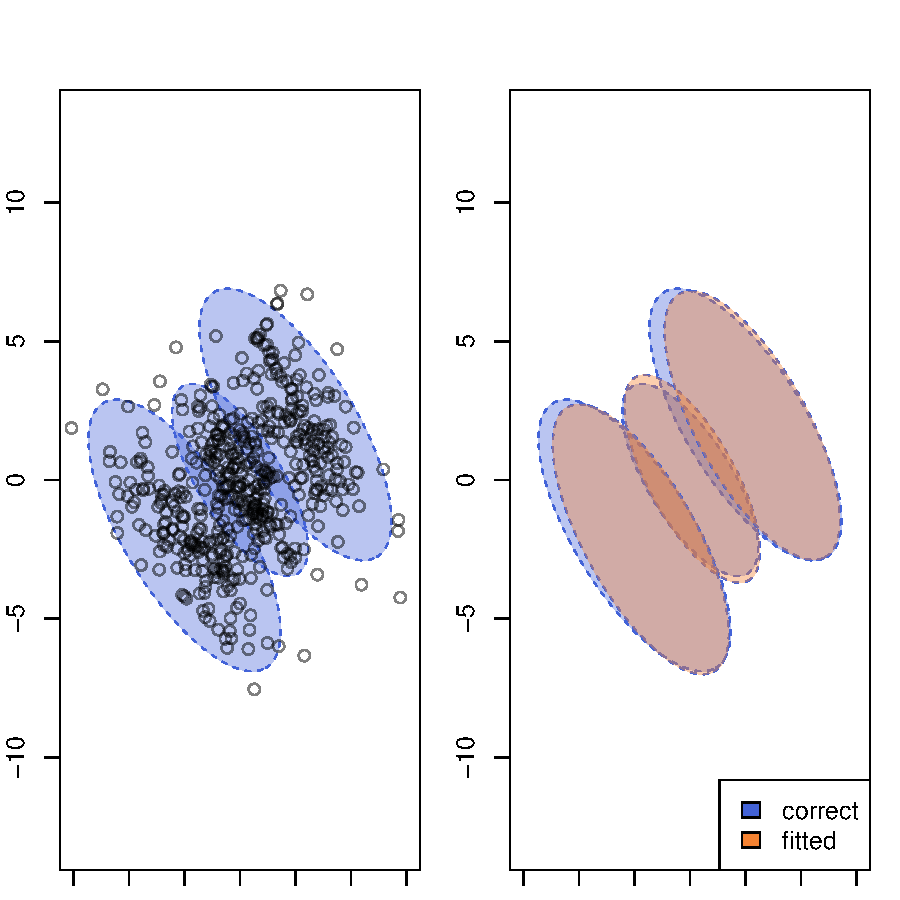
\includegraphics{chapter2-testtt}
    \caption{Correct Mixture (left) and Fitted overlayed in orange (right)}
    \label{fig:democorfit}
    \end{Rgraph}
\end{figure}
